\chapter{Implementation}

\section{Gas Costs Comparison}

In order to compare the gas consumption between implementations during testing we use eth-gas-reporter\footnote{\url{https://github.com/cgewecke/eth-gas-reporter}} which allows for to get gas usage per unit test, as well as retrieve average gas usage per method called. We configure \texttt{eth-gas-reporter} in the \texttt{truffle-config.js} file, and by prefixing a \texttt{truffle test} command with \texttt{GAS\_REPORTER=1} we can get enhanced tests as shown in Figure \ref{fig:gas-reporter}. The metrics shown in Table \ref{table:compare-gas} are obtained after running the 4 tests in the supplied \texttt{smartcontract-gascomparison} repository.

\begin{figure}[htb]
    \centering
    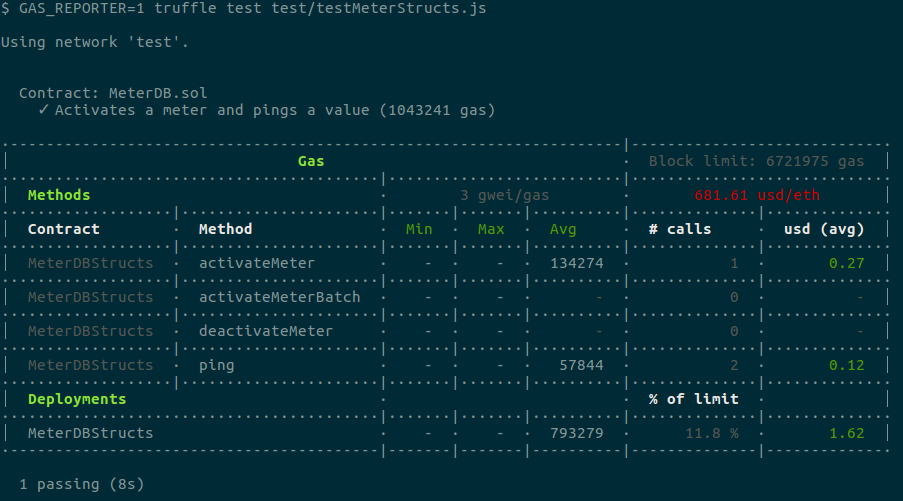
\includegraphics[width=\textwidth]{gas-reporter}
    \caption{Running a truffle test with eth-gas-reporter}
    \label{fig:gas-reporter}
\end{figure}

\section{Access Control}\label{apx:implementation:acl}

Modifiers in Solidity are used to change the behavior of functions, similarly to decorators in Python\footnote{https://www.python.org/dev/peps/pep-0318/}. The modifier in the case of Figure \ref{fig:ownable} gets called before the call to \texttt{foo()}, and after the \texttt{require} statement gets verified, execution resumes from `\texttt{\_}'.


\begin{figure}[ht!]
    \centering
    \lstinputlisting[language=Solidity]{contracts/ownership.sol}
    \caption{Using the onlyOwner modifier to enforce access control for a function}
    \label{fig:ownable}
\end{figure}

The usage of modifiers has been particularly widespread on enforcing access control to create contracts where only specific addresses can access selected privileged functions of a contract. 

In the naive case, if there were a number of smart contracts deployed by the same entity which had privileged functions callable only by an owner, the same pattern would have to be used in each contract. If a developer wanted to make the ownership check more flexible, they would have to modify the privileged members in each contract. This does not scale well, due to the number of transactions involved. In addition, if there were multiple roles, managing them on different contracts can become inefficient and has increased room for error.

We use the implementation of an Access Control List contract from DAppHub\footnote{\url{https://github.com/dapphub/ds-roles}, \url{https://github.com/dapphub/ds-auth}}. This pattern involves deploying two contracts, where one gets inherited by any contract that wishes to have access control, and the other stores all the access control list logic. 

\texttt{DSRoles.sol} allows the creation of up to 256 roles, where each role can be granted permission to call the function of a contract. 

\begin{figure}[ht!]
    \centering
    \lstinputlisting[linerange={72-84}, language=Solidity]{contracts/DSRoles.sol}
    \caption{\texttt{canCall} in \texttt{DSRoles.sol} checks if the sender is authorized to perform the function call according to the permissions set by the ACL}
    \label{fig:ownable}
\end{figure}

In order for a contract to use the ACL (\texttt{authority}), it needs to be linked with it by the owner by inheriting \texttt{DSAuth.sol} and calling the \texttt{setAuthority} function. Afterwards, any function that gets modified with \texttt{auth} will ask for permission from the linked instance of \texttt{DSRoles.sol} as shown in Figure \ref{fig:auth-mod}. This allows for a modular approach where an administrator\footnote{The version we use contains a centralized entity which handles permission. This can be re-implemented depending on the desired governance model} can grant and revoke permissions from users, depending on their clearance level.

\begin{figure}[ht!]
    \centering
    \lstinputlisting[linerange={52-67}, language=Solidity]{contracts/DSAuth.sol}
    \caption{Using the auth modifier to request permission from the linked authority (ACL)}
    \label{fig:auth-mod}
\end{figure}

\section{Listening for Events} \label{apx:implementation:events}

Events are an inexpensive way to store data in the Ethereum blockchain. An \texttt{Event} is a special kind of datatype that gets logged in the transaction receipt after a transaction gets mined. As a result, if we call a function that emits an event, that event is stored permanently in the blockchain for approximately 2000 gas. Listening for events is a fundamental process that web applications do in order to interact with a smart contract. We can also fetch all past events that a smart contract has emitted, which allows us to have a full historical log over some action that has happened in a smart contract. 

For our implementation we implemented a proof of concept script written in Javascript which can fetch all the readings that have been pinged in the smart contract, and additionally filter them by Meter Id. The same script can be implemented in Python, however there are ongoing issues with it when interacting with ganache in web3.py\footnote{\url{https://github.com/trufflesuite/ganache-cli/issues/494}}. An example is shown in Figure \ref{fig:meters-example} and the implementation is in Figure \ref{fig:get-meter-readings}.

\begin{figure}[htb]
    \centering
    \lstinputlisting{code/get_historical_readings.log}
    \caption{Retrieving all the historical readings for meters ELT01 and ELT02}
    \label{fig:meters-example}
\end{figure}

\begin{figure}[htb]
    \centering
    \lstinputlisting{code/get_meter_readings.js} 
    \caption{Script to retrieve all meter readings}
    \label{fig:get-meter-readings}
\end{figure}

